% $Id: Grid_desc.tex,v 1.24 2007/06/07 13:48:44 cdeluca Exp $
%
% Earth System Modeling Framework
% Copyright 2002-2008, University Corporation for Atmospheric Research, 
% Massachusetts Institute of Technology, Geophysical Fluid Dynamics 
% Laboratory, University of Michigan, National Centers for Environmental 
% Prediction, Los Alamos National Laboratory, Argonne National Laboratory, 
% NASA Goddard Space Flight Center.
% Licensed under the University of Illinois-NCSA License.

The ESMF Grid class is used to describe the geometry and discretization
of logically rectangular physical grids.  It also contains the
description of the grid's underlying topology and the decomposition
of the physical grid
across the available computational resources.  The most frequent 
use of the Grid class is to describe physical grids in user
code so that sufficient information is available to perform ESMF
methods such as regridding.  

\begin{center}
\begin{tabular}{|p{6in}|}
\hline
\vspace{.01in}
{\bf Key Features} \\[.01in]
Representation of grid formed by logically rectangular regions,
including uniform and rectilinear grids (e.g. lat-lon grids),
curvilinear grids (e.g. displaced pole grids), and grids formed
by connected logically rectangular regions (e.g. cubed sphere grids).\\
Support for 1D, 2D, 3D, and higher dimension grids.\\ 
Distribution of grids across computational resources for parallel
operations - users set which grid dimensions are distributed.\\
Grids can be created already distributed, so that no single
resource needs global information during the creation process.\\
Options to define periodicity and other edge connectivities either 
explicitly or implicitly via shape shortcuts.\\ 
Options for users to define grid coordinates themselves or call
prefabricated coordinate generation routines for standard grids.\\
Options for incremental construction of grids.\\
Options for using a set of pre-defined stagger locations or for setting
custom stagger locations.\\ [.03in] \hline
\end{tabular}
\end{center}

\subsubsection{Grid Representation in ESMF}

ESMF Grids are based on the concepts described in {\it A Standard Descriptor of Grids Used in Earth System Models} [Balaji 2006].  In this document
Balaji introduces the mosaic concept as a means of describing
a wide variety of Earth system model grids.  A {\bf mosaic} is
composed of grid tiles connected at their edges.  Mosaic grids
includes simple, single tile grids as a special case.  

The ESMF Grid class is a representation of a mosaic grid.  Each ESMF
Grid is constructed of one or more logically rectangular {\bf Tiles}.
A Tile will usually have some physical significance (e.g. the region
of the world covered by one face of a cubed sphere grid).

The piece of a Tile that resides on one DE (for simple cases, a DE
can be thought of as a processor - see section on the DELayout)
is called a {\bf LocalTile}.  For example, the six faces of a cubed
sphere grid are each Tiles, and each Tile can be divided into many
LocalTiles.  

Every ESMF Grid contains a DistGrid object, which defines the Grid's
index space, topology, distribution, and connectivities.  It enables
the user to define the complex edge relationships of tripole and other
grids.  The DistGrid can be created explicitly and passed into a Grid
creation routine, or it can be created implicitly if the user takes
a Grid creation shortcut.  Options for grid creation are described in 
more detail in section \ref{sec:gridcreateoptions}

\subsubsection{Supported Grids}

The range of supported grids in ESMF can be defined by:
\begin{itemize}
\item Types of topologies and shapes supported.  ESMF supports one or
more logically rectangular grid Tiles with connectivities specified
between cells.  For more details see section \ref{sec:ShapeShortcut}.
\item Types of distributions supported.  ESMF supports  regular,
irregular, or arbitrary distributions of data.  For more details see section 
\ref{sec:desc:dist}.
\item Types of coordinates supported.  ESMF supports uniform, rectilinear,
and curvilinear coordinates.  For more details see section \ref{sec:coordspec}.
\end{itemize}

\subsubsection{Grid Topologies and Periodicity}
\label{sec:ShapeShortcut}
ESMF has shortcuts for the creation of standard Grid topologies 
or{\bf shapes} up to 3D.  In many cases, these enable the user to
bypass the step of creating 
a DistGrid before creating the Grid.  The basic call is 
{\tt ESMF\_GridCreateShape()}.  With this call, the user can specify for
each dimension whether there is no connection, it is periodic, it
is a pole, or it is a bipole.  Connectivities are specified using the
ESMF\_GridConn parameter, which has values such as ESMF\_GRIDCONN\_PERIODIC.

The table below shows the ESMF\_GridConn settings used to create 
standard shapes using the ESMF\_GridCreateShape() call.  Two values
are specified for each dimension, one for the low end and one for 
the high end of its index values.

\medskip
\begin{tabular}{|l|c|c||c|c||}
\hline
& {\bf connDim1(1)} & {\bf connDim1(2)}  & {\bf connDim2(1)} & {\bf connDim2(2)}  \\
\hline
{\bf Rectangle}  & NONE & NONE & NONE & NONE \\
{\bf Bipole Sphere} & POLE & POLE & PERIODIC & PERIODIC \\
{\bf Tripole Sphere} & POLE & BIPOLE & PERIODIC & PERIODIC \\
{\bf Cylinder} & NONE & NONE & PERIODIC & PERIODIC \\
{\bf Torus}  & PERIODIC & PERIODIC & PERIODIC & PERIODIC \\
\hline
\hline
\end{tabular}
\medskip

If the user's grid shape is too complex for an ESMF shortcut routine,
or involves more than three dimensions, a DistGrid can be created
to specify the shape in detail.  This DistGrid is then passed
into a Grid create call.

\subsubsection{Grid Distribution}
\label{sec:desc:dist}

ESMF Grids have several options for data distribution (also referred to
as decomposition).  The user specifies which dimensions 
are to be distributed through a coordinate dependency (coordDep)
argument.

The main distribution options are block, regular and arbitrary.
A {\bf block} distribution is one in which the same number of
contiguous grid points are assigned to each DE in the
distributed dimension.  A {\bf regular} distribution is one in which
unequal numbers of contiguous gridpoints are assigned to each
DE in the distributed dimension.  An {\bf arbitrary} distribution is
one in which any gridpoint can be assigned to any DE.  Any ofthese
distribution options can be applied to any of the grid shapes (i.e.,
rectangle) or types (i.e., rectilinear).

Figure \ref{fig:GridDecomps} illustrates options for distribution.
\begin{figure}
\scalebox{0.9}{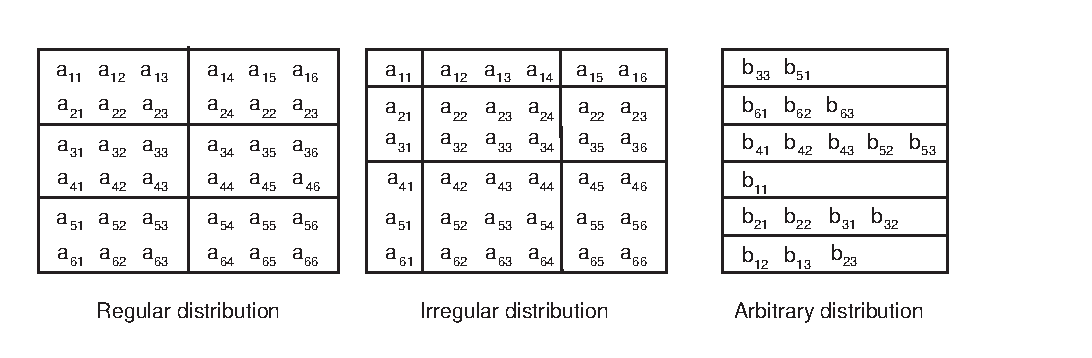
\includegraphics{GridDecomps}}
\caption{Examples of block and regular decompositions for
a 6x6 matrix {\bf a}, and an arbitrary decomposition for a 6x3 matrix {\bf b}.}
\label{fig:GridDecomps}
\end{figure}

A distribution can also be specified using the DistGrid.  This
DistGrid is then passed into a Grid create call.

\subsubsection{Grid Coordinates}
\label{sec:coordspec}
Grid Tiles can have uniform, rectilinear, or curvilinear
coordinates.  The coordinates of {\bf uniform} grids are equally spaced along their axes, and can be fully specified by the coordinates of the two opposing points
that define the grid's physical span.  The coordinates of {\bf rectilinear} grids
are unequally spaced along their axes, and can be fully specified by giving
the spacing of grid points along each axis.  The coordinates of {\bf curvilinear 
grids} must be specified by giving the explicit set of coordinates for each
grid point.  Curvilinear grids are often uniform or rectangular grids that 
have been warped; for example, to place a pole over a land mass so that it
does not affect the computations performed on an ocean model grid.  Figure
\ref{fig:LogRectGrids} shows examples of each type of grid.

Any of these logically rectangular grid types can be combined through edge
connections to form a mosaic.  Cubed sphere and yin-yang grids are examples
of mosaic grids.
 
\begin{figure}
\scalebox{0.9}{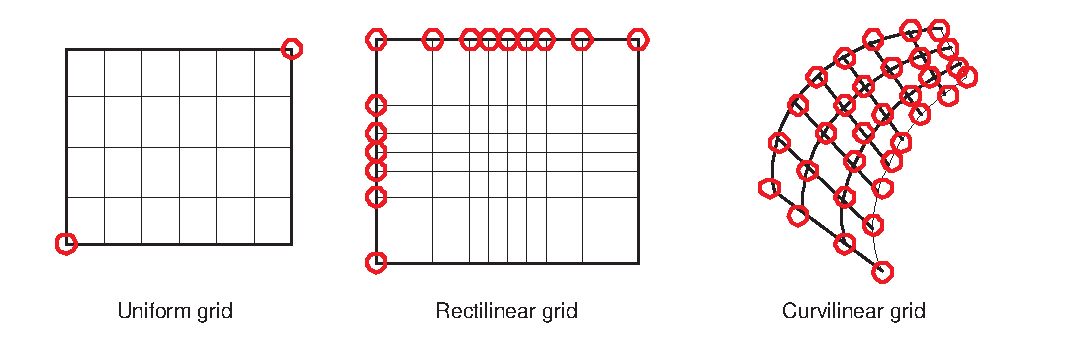
\includegraphics{LogRectGrids}}
\caption{Types of logically rectangular grid tiles.  Red circles show the
values needed to specify grid coordinates for each type.}
\label{fig:LogRectGrids}
\end{figure}

Each of these coordinate types can be set for each of the standard grid shapes
described in section \ref{sec:ShapeShortcut}.  

The table below shows how examples of common single Tile grids fall 
into this shape and coordinate taxonomy.  Note that any
of the grids in the table can have a regular or arbitrary distribution.

\medskip
\begin{tabular}{|p{.9in}|p{1.7in}|p{1.7in}|p{1.7in}|}
\hline
 & {\bf Uniform} & {\bf Rectilinear} & {\bf Curvilinear} \\ 
\hline
{\bf Sphere} & Global uniform lat-lon grid & Gaussian grid & Displaced pole grid \\
\hline
{\bf Rectangle} & Regional uniform lat-lon grid & Gaussian grid section & Polar stereographic grid section\\
\hline
\end{tabular}

\subsubsection{Coordinate Specification and Generation}

There are two ways of specifying coordinates in ESMF.  The
first way is for the user to {\bf set} the coordinates.  The second 
way is to take a shortcut and have the framework {\bf generate}
the coordinates.  

The only ESMF generation routine currently available is for uniform grids.

See Section~\ref{sec:usage:coordstore} for more description and examples of
setting coordinates.

\subsubsection{Staggering}

A useful finite difference technique is to place different physical
quantities at different locations within a grid cell. This {\bf staggering}
of the physical variables on the mesh is introduced so that the difference
of a field is naturally defined at the location of another variable. 

The ESMF Grid class supports a wide variety of stagger locations, including
those sufficient to specify any of the standard Arakawa staggers. The 
Grid supports staggers located at cell centers, corners, edges, 
faces, and in 3D and higher dimensions. The user may specify
common stagger locations using predefined values, or may construct
custom ones for cases that the predefined values don't cover.

As a default the ESMF Grid class provides symmetric staggering, so
that cell centers are enclosed by cell perimeter (e.g. corner) 
stagger locations. This means the coordinate arrays for
some stagger locations may be padded to one element larger in some
dimensions than the cell center arrays to allow the enclosure. 
However, to achieve other types of staggering, the user may alter 
or eliminate this padding by using the appropriate options when adding
a stagger location to a Grid. 
 
For examples and a full description of the stagger interface 
please see Section~\ref{sec:usage:staggerloc}. 

\subsubsection{Stages in Grid Creation} 
\label{sec:gridcreatestages}

In ESMF there are two stages to Grid creation.
\begin{enumerate}
\item Creation of the Grid shape.  At the completion of this
stage, the Grid has a specific topology and distribution, but
empty coordinate arrays.  The Grid can be used as the basis for
allocating a Field.
\item Specifying the Grid coordinates and any other information
required for regridding (this can vary depending on the particular
regridding method).  At the completion of this stage, the Grid can
be used in a regridding operation.
\end{enumerate}
There are shortcut methods in ESMF for both stages.

Each stage has at least one ESMF call, and depending on 
whether shortcuts are used or not, may have more.
This gives the user the opportunity to trade off the 
ease of using a prefabricated grid with the flexibility 
of building a highly customized grid.  Incremental
construction can also be useful when distributing a grid object
before setting its coordinates, or when multiple components
contribute to the definition of a grid. 

\subsubsection{Options for Grid Creation}
\label{gridcreateoptions}

The following chart shows typical creation calls and 
sequences.  

\medskip
\begin{tabular}{|p{2.6in}|p{1in}|p{1in}|p{1.4in}|}
\hline
\multicolumn{4}{|l|}{{\bf Options for Grid Creation}} \\
\hline
Command sequence & Missing & Function & ESMF\_GRIDSTATUS\_ \\ 
\hline
ESMF\_GridCreateEmpty() 
& Topology information and coordinates, other options undefined
& A Grid object shell is allocated but space for 
internal objects is not
& NOT\_READY \\
\hline
ESMF\_GridCreate(distGrid)\newline
{\bf or} \newline
ESMF\_GridCreateEmpty()\newline
ESMF\_GridSet(distGrid)\newline
...\newline
ESMF\_GridCommit(\newline
\hspace{.1in} ESMF\_GRIDSTATUS\_SHAPE\_READY)\newline
{\bf or use a shortcut} \newline
ESMF\_GridCreateShape()\newline
& Space for coordinates is allocated but coordinate
values are not set
& Can be used as the basis for Field allocation
& SHAPE\_READY\\
\hline
ESMF\_GridCreate(distGrid)\newline
ESMF\_GridSetCoordFromArray()\newline
ESMF\_GridCommit(\newline
\hspace{.1in} ESMF\_GRIDSTATUS\_REGRID\_READY)\newline
{\bf or} \newline 
ESMF\_GridCreate(distGrid)\newline
ESMF\_GridLocalTileGet(localTile)\newline
... user fills in localTile coordinate values
ESMF\_GridCommit(\newline
\hspace{.1in} ESMF\_GRIDSTATUS\_REGRID\_READY)\newline
{\bf or use a shortcut} \newline
ESMF\_GridCreateShape()\newline
ESMF\_GridGenCoordUni()\newline
ESMF\_GridCommit(\newline
ESMF\_GRIDSTATUS\_REGRID\_READY)
& Nothing; Grid is complete
& Can be used in regrid methods
& REGRID\_READY\\
\hline
\end{tabular}



 


